\section{DSL Examples}
\label{sec:Examples}

This Section presents three simple \DSMLs, namely \textsf{PacMan}, Finite State
Machines (\textsf{FSM}), and Petri Nets (\textsf{PN}), following the same 
presentation:
\begin{itemize}
	\item The \DSL's structure is specified using a metamodel expressed in \MOF;
   we also informally specify a possible \emph{concrete syntax}, then provide a 
   simple witness model.

   \item The \DSL's semantics is sketched, without details of implementations that
   highly depend on the MTL, and the modelling style of the MT designer. We however
   show for the \textsf{PacMan} example how a similar approach in various MTLs 
   may lead to a similar MT structure, independently of the underlying MTL.

   \item A set of animations are then described in detail, and numbered for 
   future reference.
\end{itemize}
Note that we assume that the \DSL structure follows the Executable \DSML Pattern
\citep{Combemale-Cregut-Pantel:2012}, which consists of two separate metamodels for
defining executable \DSMLs:
\begin{itemize}
	\item The so-called \emph{Domain Definition} metamodel captures the 
   \emph{static} structure of the \DSL, which typically serves for defining valid
   models using various textual and/or visual syntaxes;
   
   \item The \emph{State Definition} metamodel adds new information on top of the
   Domain Definition metamodel to enable state-based execution, thus defining those
   elements that are modified during execution.
\end{itemize}
Both metamodels typically need to be merged, using different techniques (e.g.,
using \MOF's ``package merge'' approach \cite{TR:OMG-MOF:2016}, or other 
composition techniques \cite{J:Abouzahra-Sabraoui-Afdel:2020}).
For clarity and presentation simplification purposes, we depicts both metamodels
in a merged fashion, although we visually distinguish each part: the Domain Definition
metamodel elements are represented using the regular font with plain arrows for 
references; while the State Definition elements use curvy fonts and dotted references.

\subsection{\textsf{PacMan}: A \DSL for the PacMan game}
\label{sec:Examples:PacMan}

The PacMan game is a popular arcade game that gained interest in the \MDE community
because it captures a well-known, simple reactive \DSL with an easily understandable
concrete syntax, and presents interesting real-time features for execution. 

\subsubsection{Specification}
\label{sec:Examples:PacMan:Specification}

On the top left compartment is represented a metamodel
$\mathsf{MM}_{\mathsf{PM}}$, as created by a DSL engineer. A \textsf{Game} 
consists of a sequence of \textsf{Level}s, each displaying a \textsf{Maze} where
\textsf{Persona}s evolve. A \textsf{Level} terminates when \textsf{PacMan} is eaten
by a \textsf{Ghost}, or when it has eaten all \textsf{Cookie}s. Several players
may compete for the highest \textsf{Score}.

On the top right compartment, a basic model $\mathsf{M}_{\mathsf{2x2}}$ with a
\textsf{unique} \textsf{Level} of size 2x2, as possibly created by a modeller,
is depicted using three different concrete syntaxes:
textual for $^{\mathsf{TXT}}\mathsf{M}_{\mathsf{2x2}}$ (inspired by eMotions 
\cite{J:RiveraDuranVallecillo:2009}); based on UML Object Diagram for
\cite{B:Rumbaugh-Jacobson-Booch:2004} for $^{\mathsf{OD}}\mathsf{M}_{\mathsf{2x2}}$;
and freely inspired by the real game for $^{\mathsf{Viz}}\mathsf{M}_{\mathsf{2x2}}$,
the two latters being graphical.

\begin{figure*}[t]
   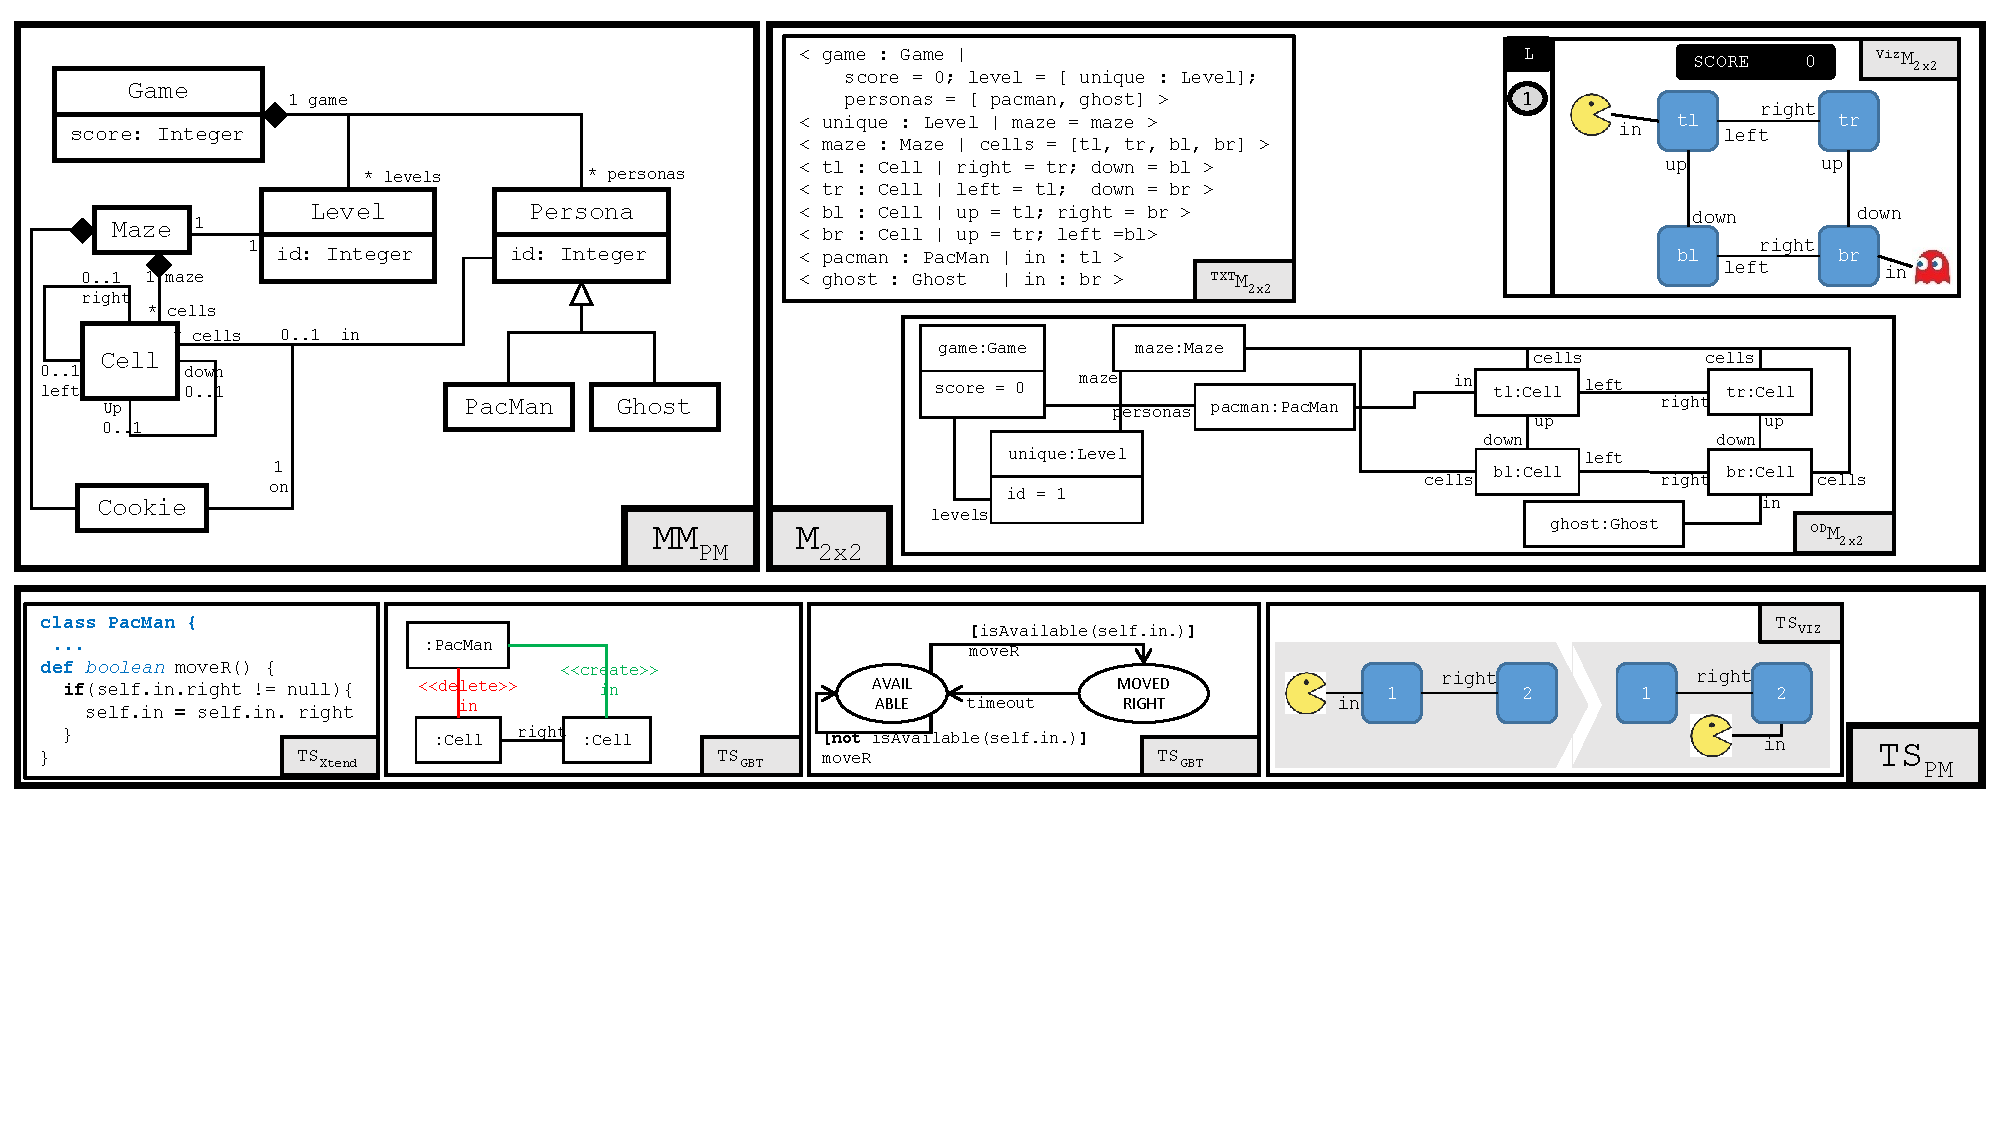
\includegraphics[width=\textwidth,clip, trim=0cm 5.5cm 0cm 0cm]{MM-M-T.pdf}
   \caption{Specifying a Pac-Man DSL: the DSL engineer create the metamodel 
   $\mathsf{MM}_{\mathsf{PM}}$; a modeller chooses a concrete syntax to create
   a simple model $\mathsf{M}_{\mathsf{2x2}}$; a MT designer specifies a transformation
   $\mathsf{TS}_{\mathsf{PM}}$ (only the \emph{\textsf{moveR}} MT unit is shown)}
   \label{fig:PacMan}
   \Description[<short description>]{<long description>}
\end{figure*}

\subsubsection{Execution}
\label{sec:Examples:PacMan:Execution}

The bottom compartment of \autoref{fig:PacMan} describes a simple rule 
\emph{\textsf{moveR}} (moving Pac-Man on a \textsf{Cell} at its right, if 
available) as part of the simulation MT specification $\mathsf{TS}_{\mathsf{PM}}$,
as part of $\mathsf{MM}_{\mathsf{PM}}$'s executable semantics. 
The first MT, $\mathsf{TS}_{\mathsf{Xtend}}$, uses metaprogramming 
(based on Xtend with GeMoC \cite{Leroy-Bousse-etAl:2017}). The next and last ones
are based on Graph Transformations: $\mathsf{TS}_{\mathsf{GBT}}$ relies on 
$^{\mathsf{OD}}\mathsf{M}_{\mathsf{2x2}}$ to express the rewriting (as would be 
expressed e.g. in Henshin \cite{Bill-Gabmeyer-Kaufmann-Seidl:2014}); 
while $\mathsf{TS}_{\mathsf{VIZ}}$ relies on $^{\mathsf{Viz}}\mathsf{M}_{\mathsf{2x2}}$
(as would be expressed e.g. in AtoMPM \cite{J:SyrianiVangheluwe:2013}). 
Finally, $\mathsf{TS}_{\mathsf{FSM}}$ presents an MT fragment expressed with 
a UML's Finite State Machine \cite{B:Rumbaugh-Jacobson-Booch:2004}. 
Note that all MT specifications (fragments) but $\mathsf{TS}_{\mathsf{Xtend}}$ 
present a graphical representation, showing that MT specifications may well be 
graphically visualised as well.

\subsubsection{Animations}
\label{sec:Examples:PacMan:Animations}

The PacMan game typically uses three kinds of animations for different situations:
\begin{description}
   \item[A \textsf{Persona} moves.] Typically, a specific animation could be attached
   to each movement, as they are traditionally encoded in different rules/operations
   (cf. e.g. \textsl{moveR} as specified in \autoref{fig:PacMan}, but also 
   \textsl{moveL}, \textsl{moveU} and \textsl{moveD} for moving left, up and down).
   Depending on whether the MTL allows using abstract classes (which would be 
   \textsf{Persona} here) for MT specification, these rules/operations may need 
   to be duplicated. 
   
   \item[\textsf{PacMan} eats a \textsf{Cookie}.] This occurs when \textsf{PacMan} is on a \textsf{Cell}
   that contains a \textsf{Cookie}, making it disappear and triggering a 
   \textsf{Score} update.
   
   \item[\textsf{PacMan} is eaten by a \textsf{Ghost}.] This occurs when 
   \textsf{PacMan} is on the same \textsf{Cell} as a \textsf{Ghost}, which may occur
   by either \textsf{Persona} making a move to an already occupied \textsf{Cell}.
\end{description}
To summarise, we would have to define four different animations to fully animate
the \textsf{PacMan} \DSL:
\begin{description}
   \item[PM.1] The \textsf{Persona} disappears from one \textsf{Cell} and reappears
   on another (adjacent) \textsf{Cell}.
   
   \item[PM.2] Assuming \textsf{PacMan} is on a \textsf{Cell} containing a \textsf{Cookie},
   the \textsf{Cookie} disappears.
   
   \item[PM.3] The \textsf{Score} is updated by a given increment. 

   \item[PM.4] Assuming \textsf{PacMan} and a \textsf{Ghost} are on the same
   \textsf{Cell}, \textsf{PacMan} disappears.
\end{description}
Note that those animations are not completely unrelated. First, \textbf{PM.2} and
\textbf{PM.3} need to be conducted sequentially quickly enough to not notice a
time gap. Second, \textbf{PM.2} and \textbf{PM.4} appear to be very similar in
nature: they both assume that two objects are located on the same \textsf{Cell} 
before making one of them disappear.

\subsection{\textsf{FSM}: A \DSL for Finite-State Machines}
\label{sec:Examples:FSM}

Finite State Machines (FSM) represent a common \DSL for capturing state-based 
behaviour of various biological, but also computational domains (e.g. Turing 
Machines, but also Chomsky's Regular Grammars, among others). This Section considers
FSMs that are simplified in various ways: in particular, we only consider a
word acceptance semantics where transitions do not contain guards and triggers are
reduced to their simplest expression, namely simple strings.

\subsubsection{Specification}
\label{sec:Examples:FSM:Specification}

\begin{figure}%
   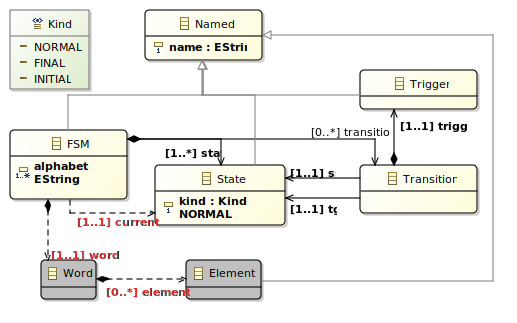
\includegraphics[width=\columnwidth]{FSM}%
   \caption{A metamodel for Finite State Machines.}%
   \label{fig:FSM_MM}%
\end{figure}


\autoref{fig:FSM_MM} (top) specifies the metamodel of the Finite State Machine \DSL. 
An \textsf{FSM} is composed of \textsf{State}s identified by a \textsf{name}, and
\textsf{Transition}s that contain a simple \textsf{Trigger}, specified as 
\textsf{name}d event. \autoref{fig:FSM_M} depicts a simple model consisting of 
three \textsf{State}s and three \textsf{Transition}s, to recognise the regular 
expression $\mathtt{(a\cdot b)^\star\ b}$. 

We assume the classical visual representation for \textsf{FSM}: a \textsf{State}
is represented by a circle labelled with its \textsf{name}; and a 
\textsf{Transition} is represented by an arrow pointing to its \textsf{tgt} and 
carrying the \textsf{Trigger}'s name as a label. We represent the \textsf{current}
\textsf{State} by surimposing a red rounded form (that we call \emph{token}) over
the corresponding \textsf{State} (cf. \autoref{fig:FSM_M}).


\subsubsection{Execution}
\label{sec:Examples:FSM:Execution}

We adopt a \emph{word-recognising} semantics encoded in a transformation called
\textsf{accept} that reads a \textsf{Word} and traverses the \textsf{FSM}. A 
\textsf{Word} is accepted iff the \textsf{current} \textsf{State} of the \textsf{FSM}
is \textsf{FINAL} when the \textsf{Word} becomes empty.

\subsubsection{Animations}
\label{sec:Examples:FSM:Animations}

Typically, \textsf{accept} is implemented using a sub-transformation 
\textsf{fire(e : Element) : State [0..1]} that determines which \textsf{State} 
to update to when consuming an \textsf{Element} \textsf{e}, making it a good 
candidate for four different animations, when \textsf{fire} returns an actual 
\textsf{State}:
\begin{description}
   \item[FSM.1] The token disappears from the \textsf{current} \textsf{State} and
   reappears inside the updated \textsf{current};
   \item[FSM.2] The token disappears from the \textsf{current} \textsf{State}, and
   slides along the entire arrow of the fired \textsf{Transition}, then appears in
   the updated \textsf{current};
   \item[FSM.3] The token disappears from the \textsf{current} \textsf{State}, the
   arrow of the fired \textsf{Transition} blinks in red for 2 seconds, then the 
   token reappears in the updated \textsf{current}.
\end{description}


\begin{figure}[t]%
   \centering
   \begin{subfigure}[b]{0.45\columnwidth}
      \centering
      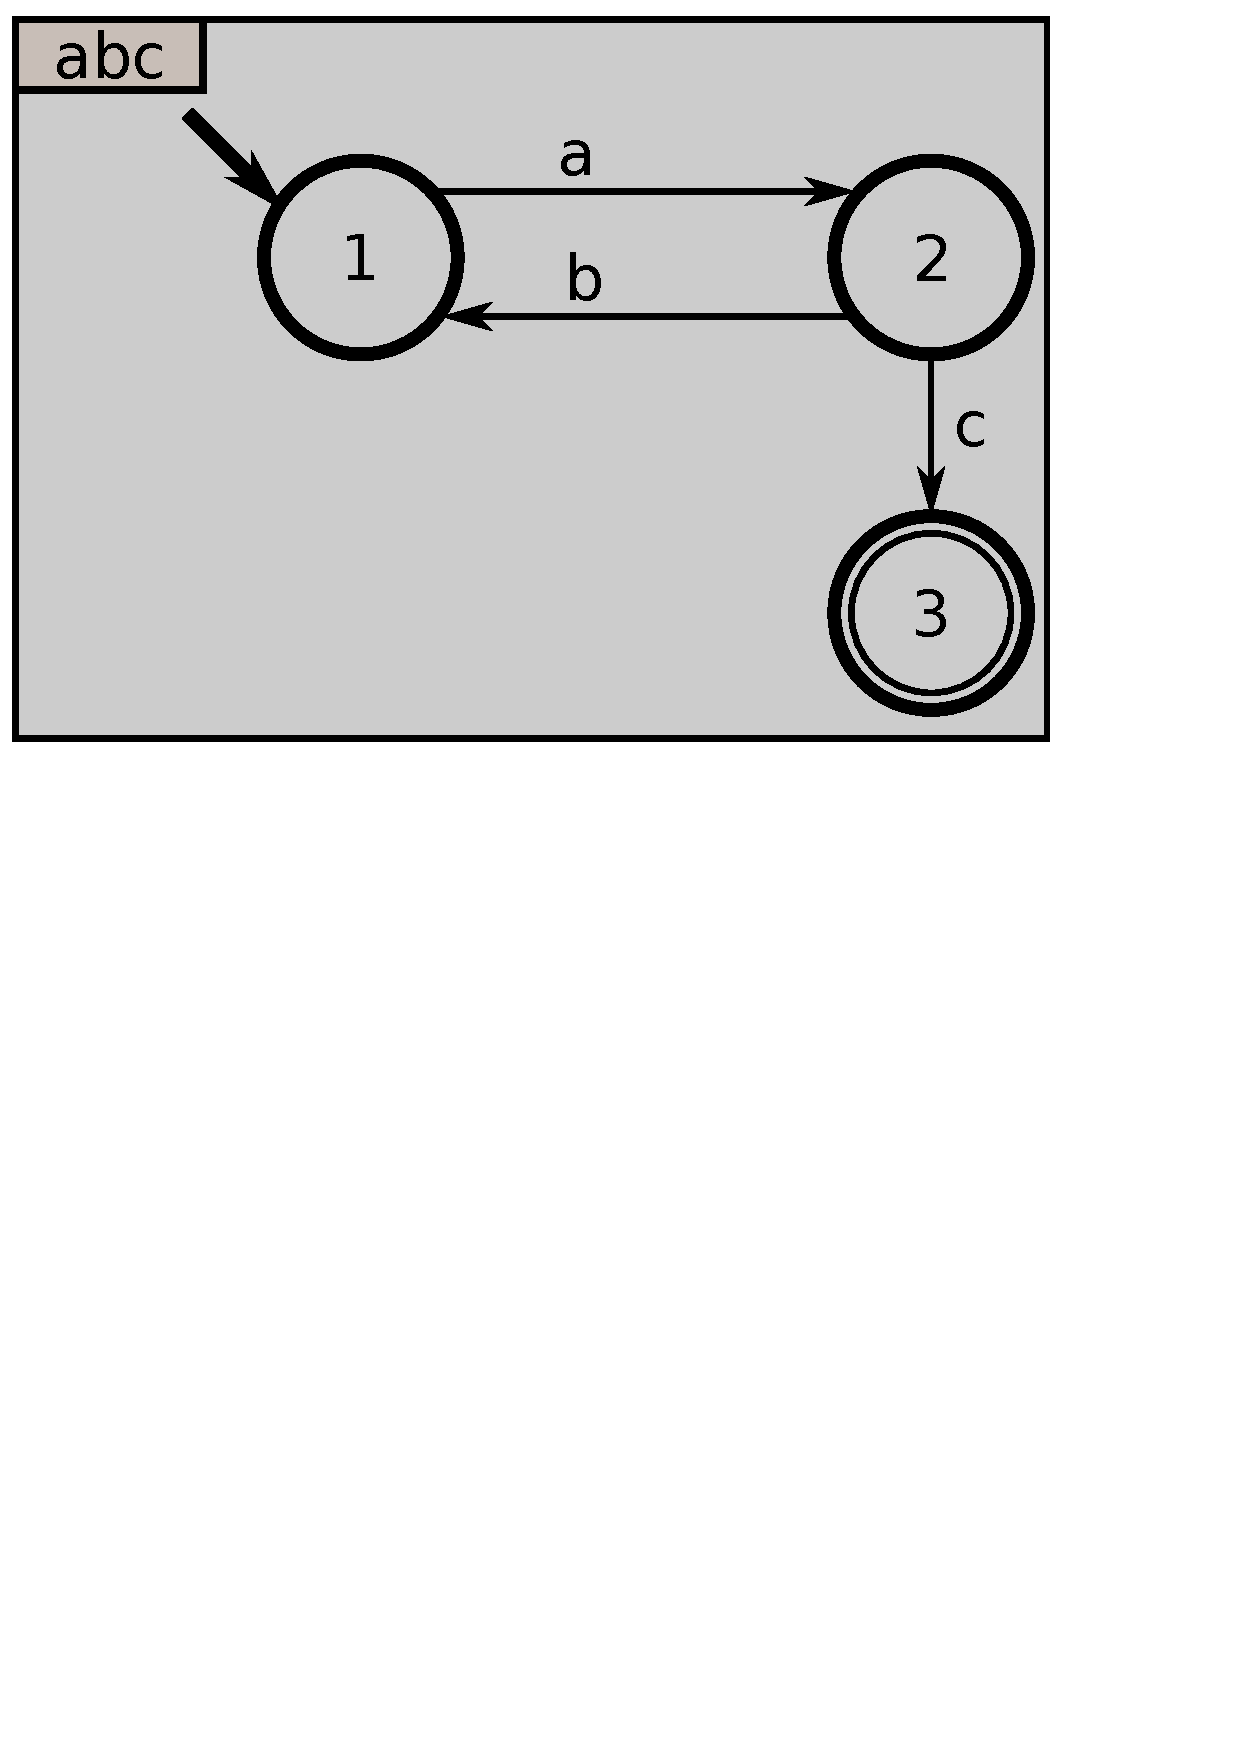
\includegraphics[width=\columnwidth, clip, trim=0cm 17cm 3cm 0cm]{FSM_M.pdf}%
      \caption{Editing \textsf{abc} to obtain a 3-state/3-transition FSM model: 
      states \textsf{1} and \textsf{3} are respectively \textsf{INITIAL} and 
      \textsf{FINAL}.}
      \label{fig:FSM:Model:Edition}
   \end{subfigure}
   \hfill
   \begin{subfigure}[b]{0.45\columnwidth}
      \centering
      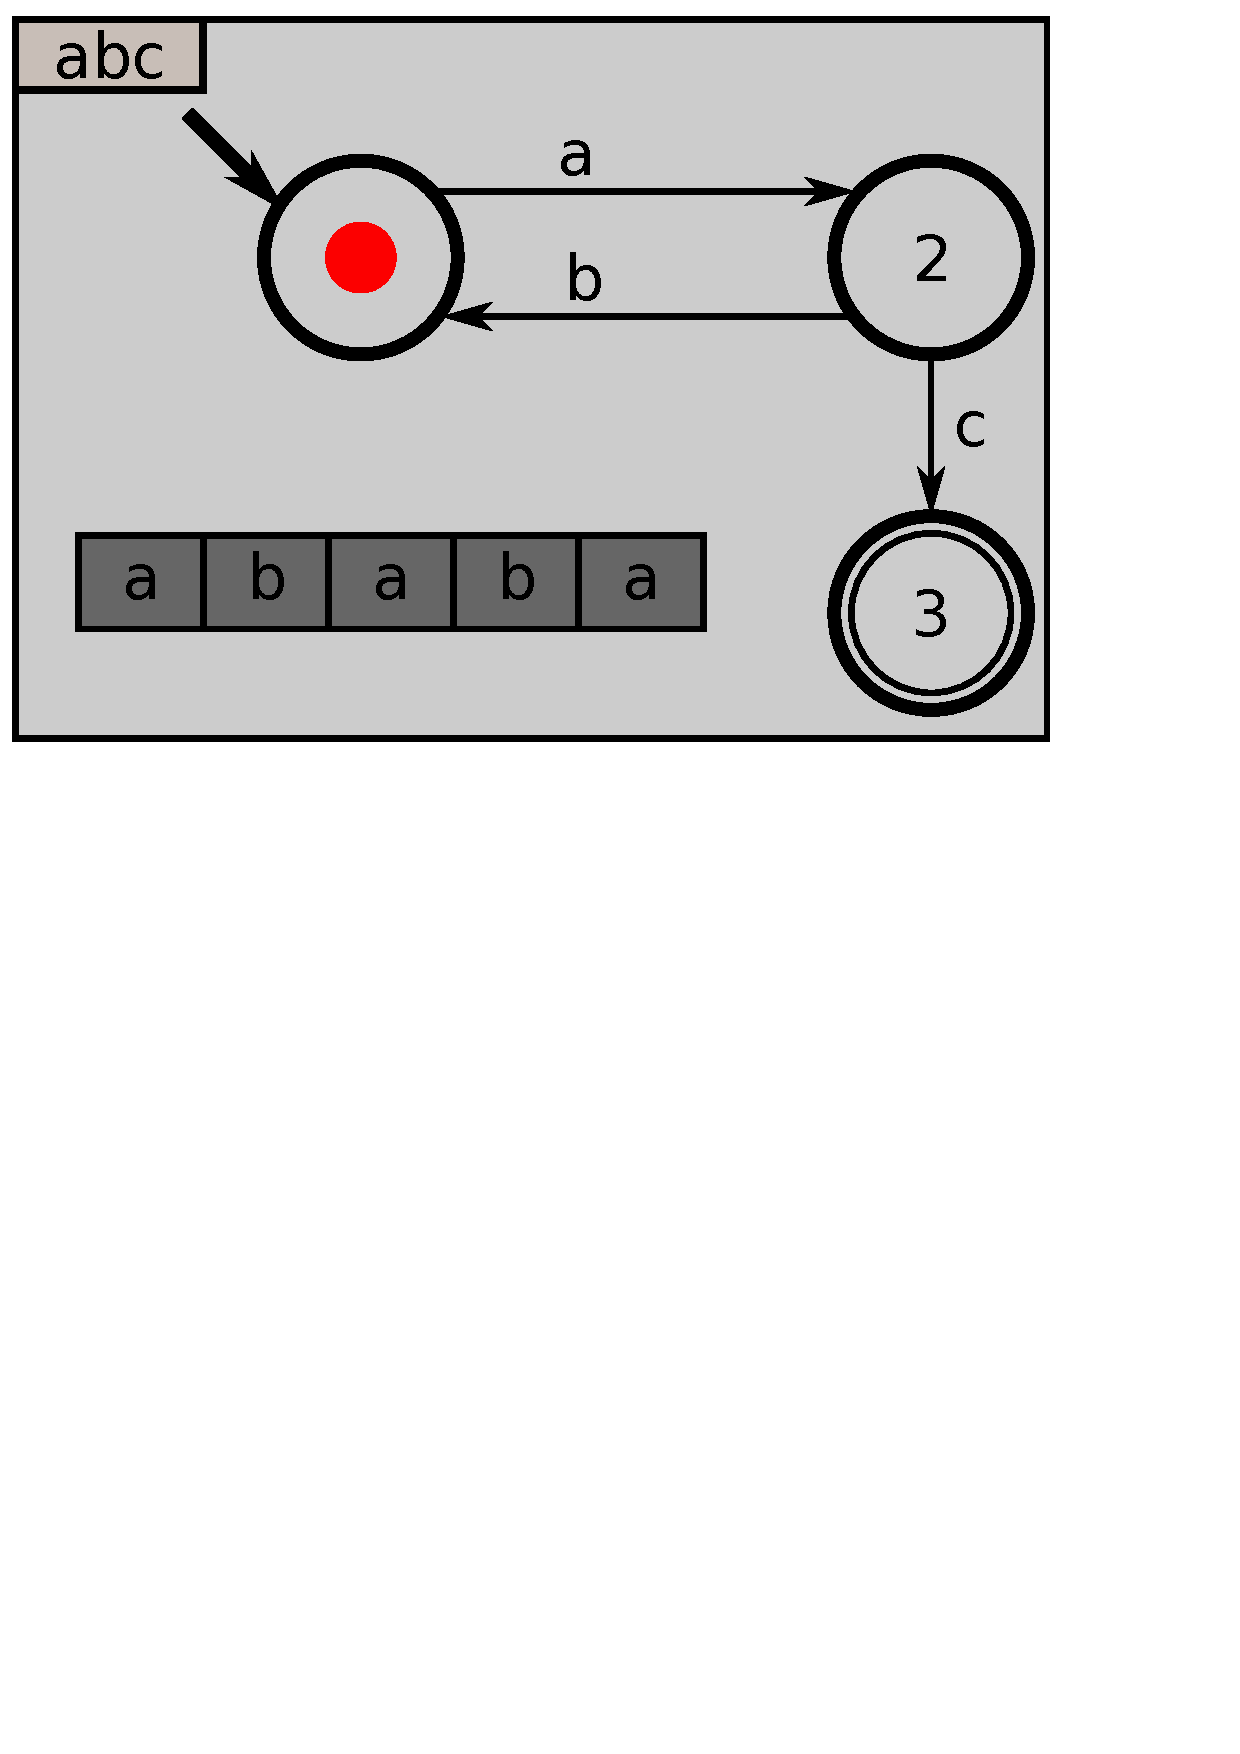
\includegraphics[width=\columnwidth, clip, trim=0cm 17cm 3cm 0cm]{FSM_MX.pdf}%
      \caption{Starting executing \textsf{abc}: the \textsf{current} 
      \textsf{State} is overlayed with a red token, and attempting to accept the
      word \textsf{ababa}.}
      \label{fig:FSM:Model:Execution}
   \end{subfigure}
  
   \vskip\baselineskip
   \begin{subfigure}[b]{0.45\columnwidth}
      \centering
      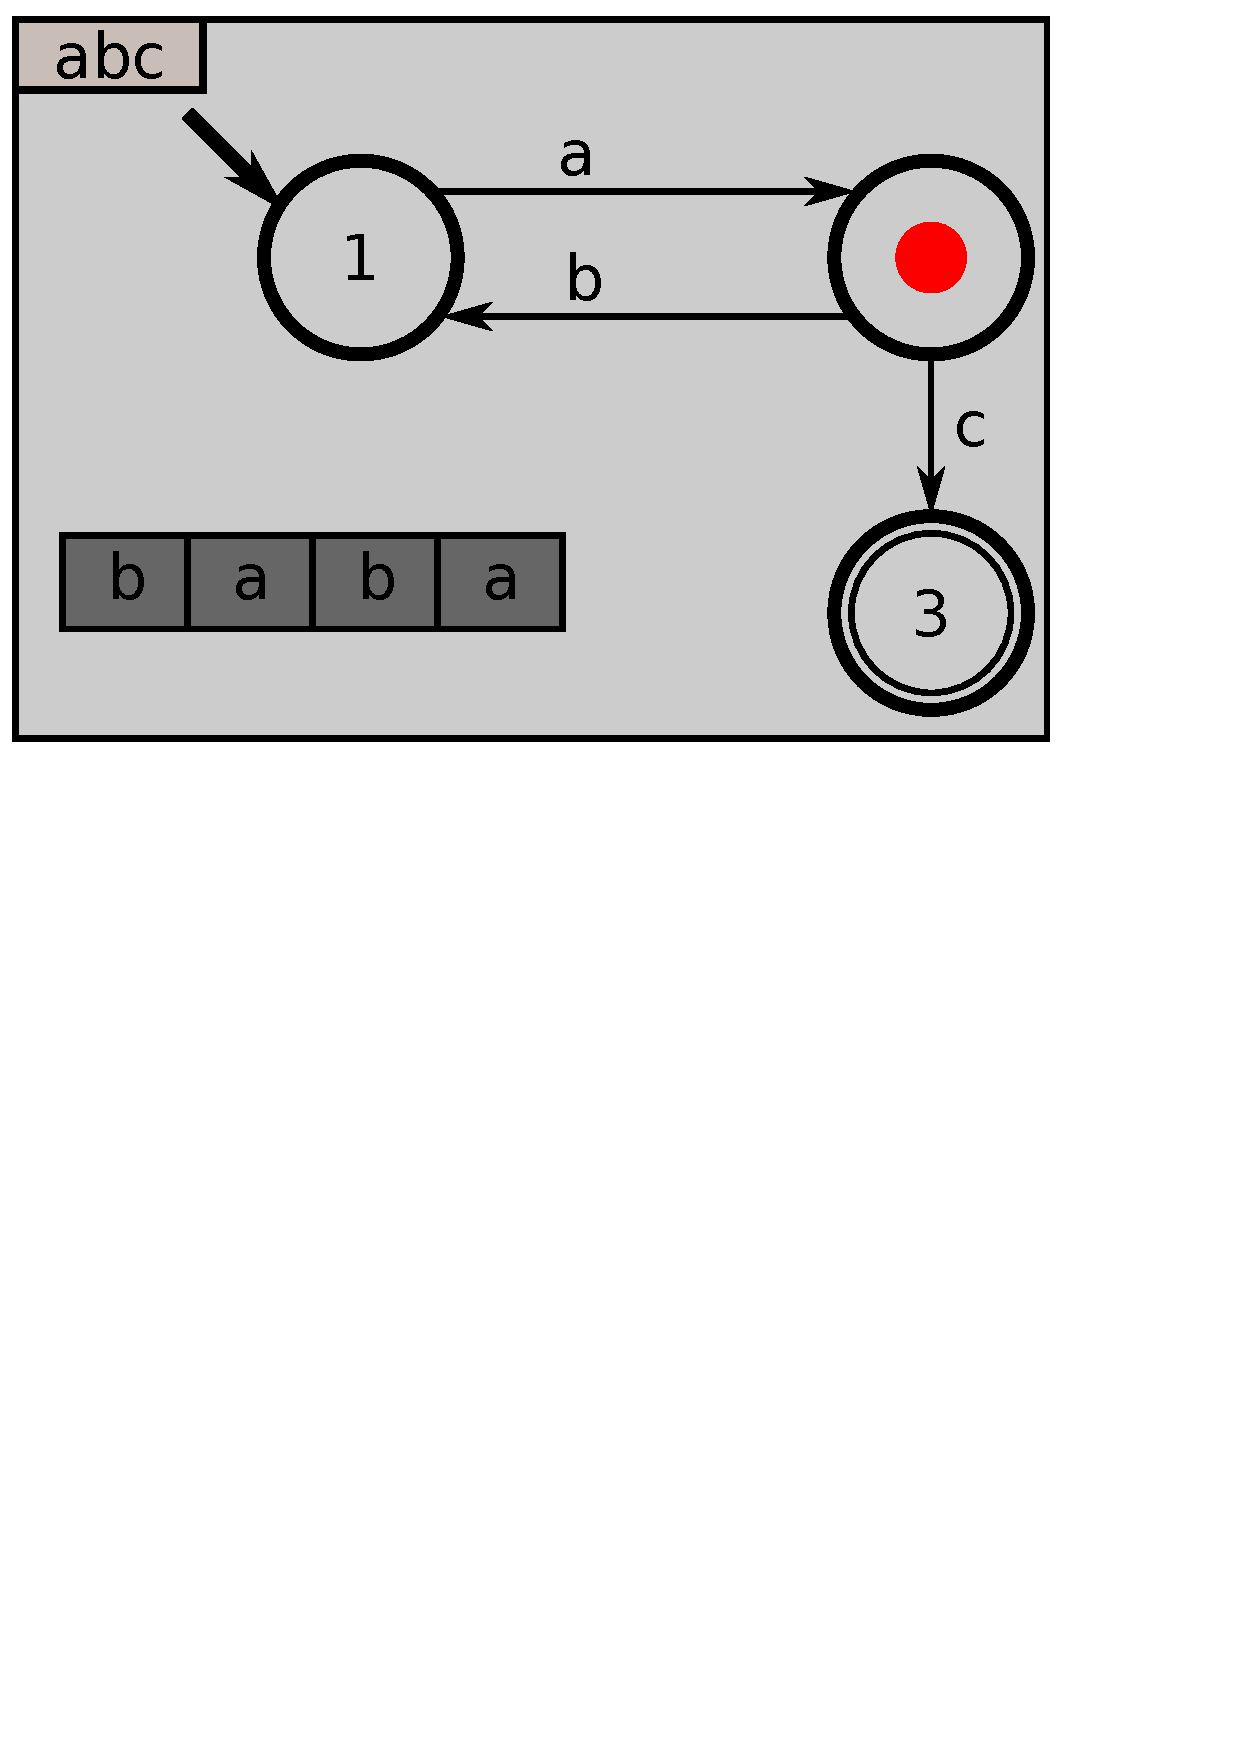
\includegraphics[width=\columnwidth, clip, trim=0cm 17cm 3cm 0cm]{FSM_MA11.pdf}%
      \caption{\textbf{Animation FSM.1:} The first execution step moves the token in
      \textsf{State} 2 (while consuming the first \textsf{Element} \textsf{a}).}
      \label{fig:FSM:Model:Animation:FSA1.1}
   \end{subfigure}
   \hfill
   \begin{subfigure}[b]{0.45\columnwidth}
      \centering
      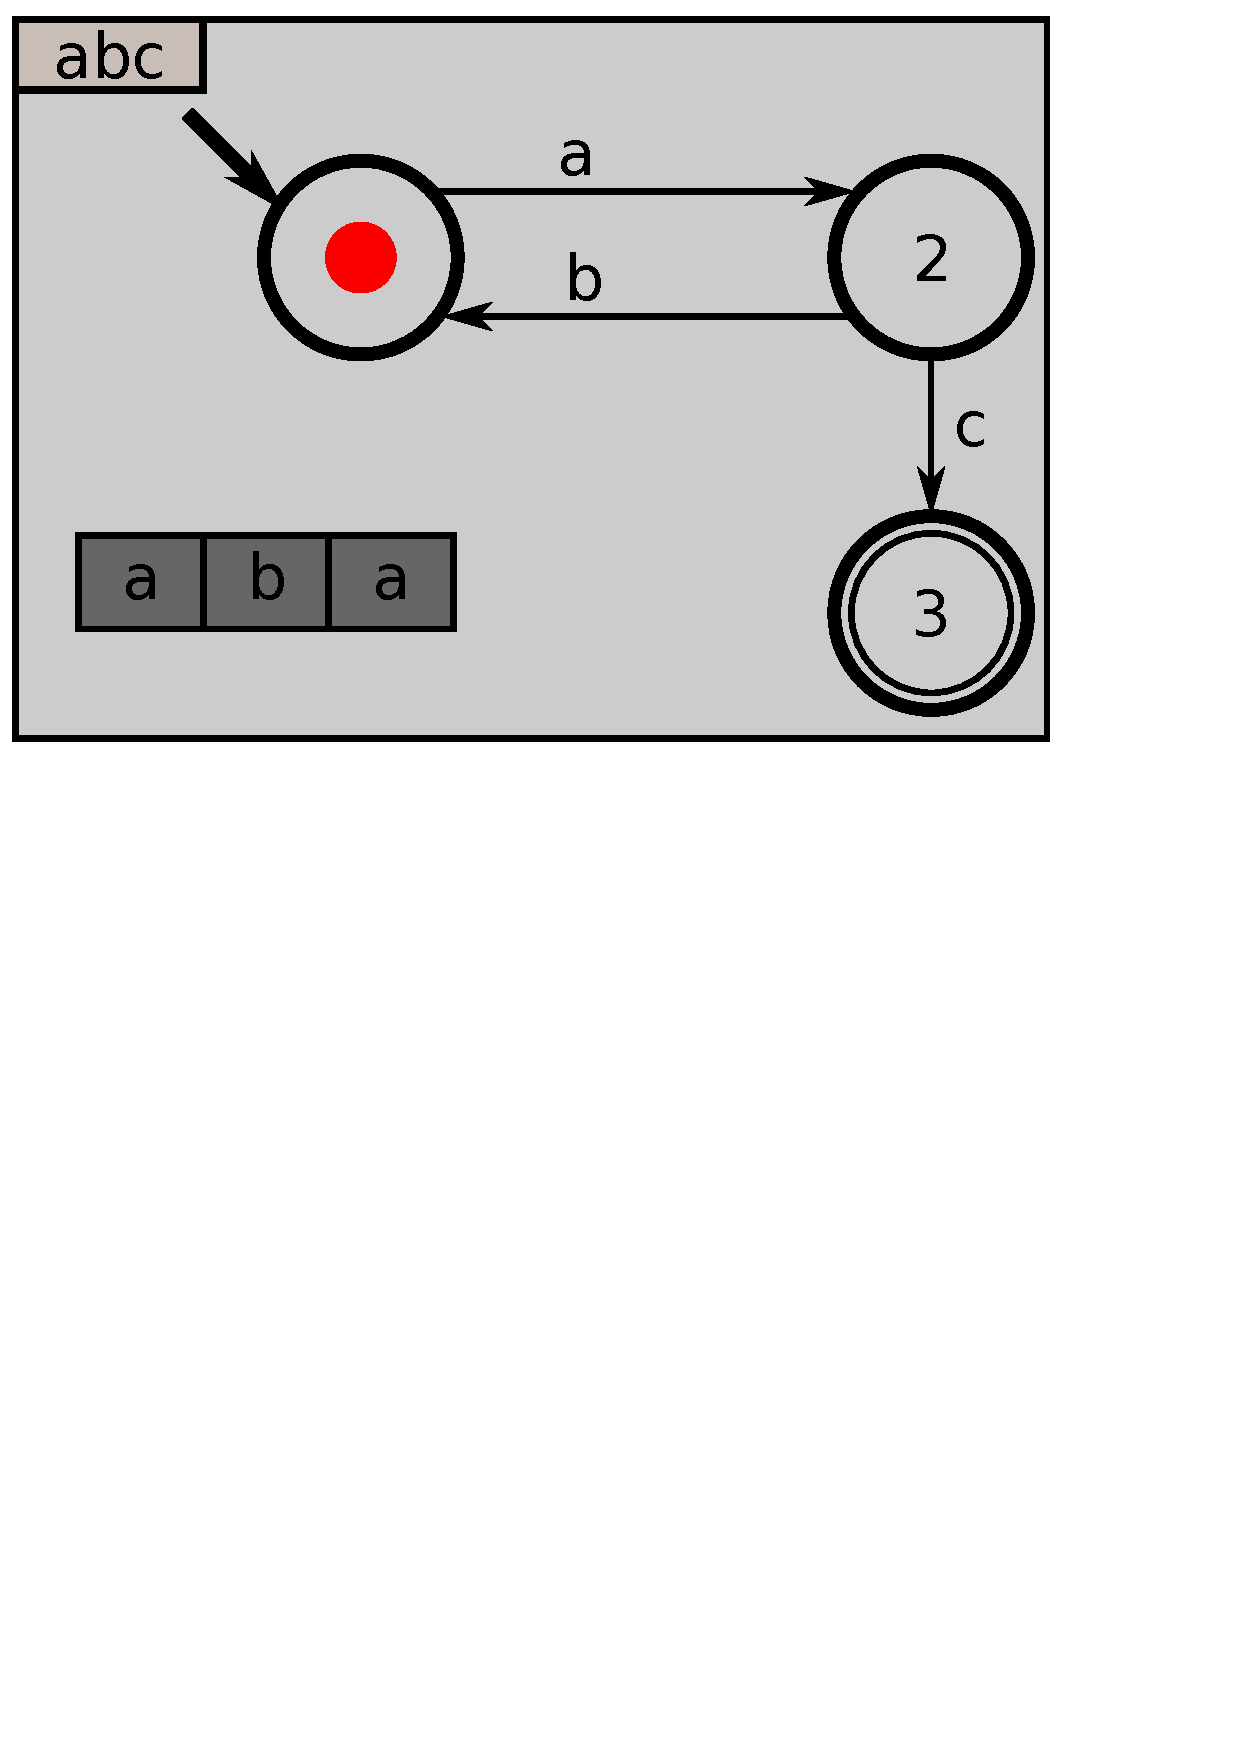
\includegraphics[width=\columnwidth, clip, trim=0cm 17cm 3cm 0cm]{FSM_MA12.pdf}%
      \caption{\textbf{Animation FSM.1:} The second execution step moves the token 
      back in \textsf{State} 1 (while consuming \textsf{b}).}
      \label{fig:FSM:Model:Animation:FSA1.2}
    \end{subfigure}
 
    \vskip\baselineskip
    \begin{subfigure}[t]{0.45\columnwidth}
      \centering
      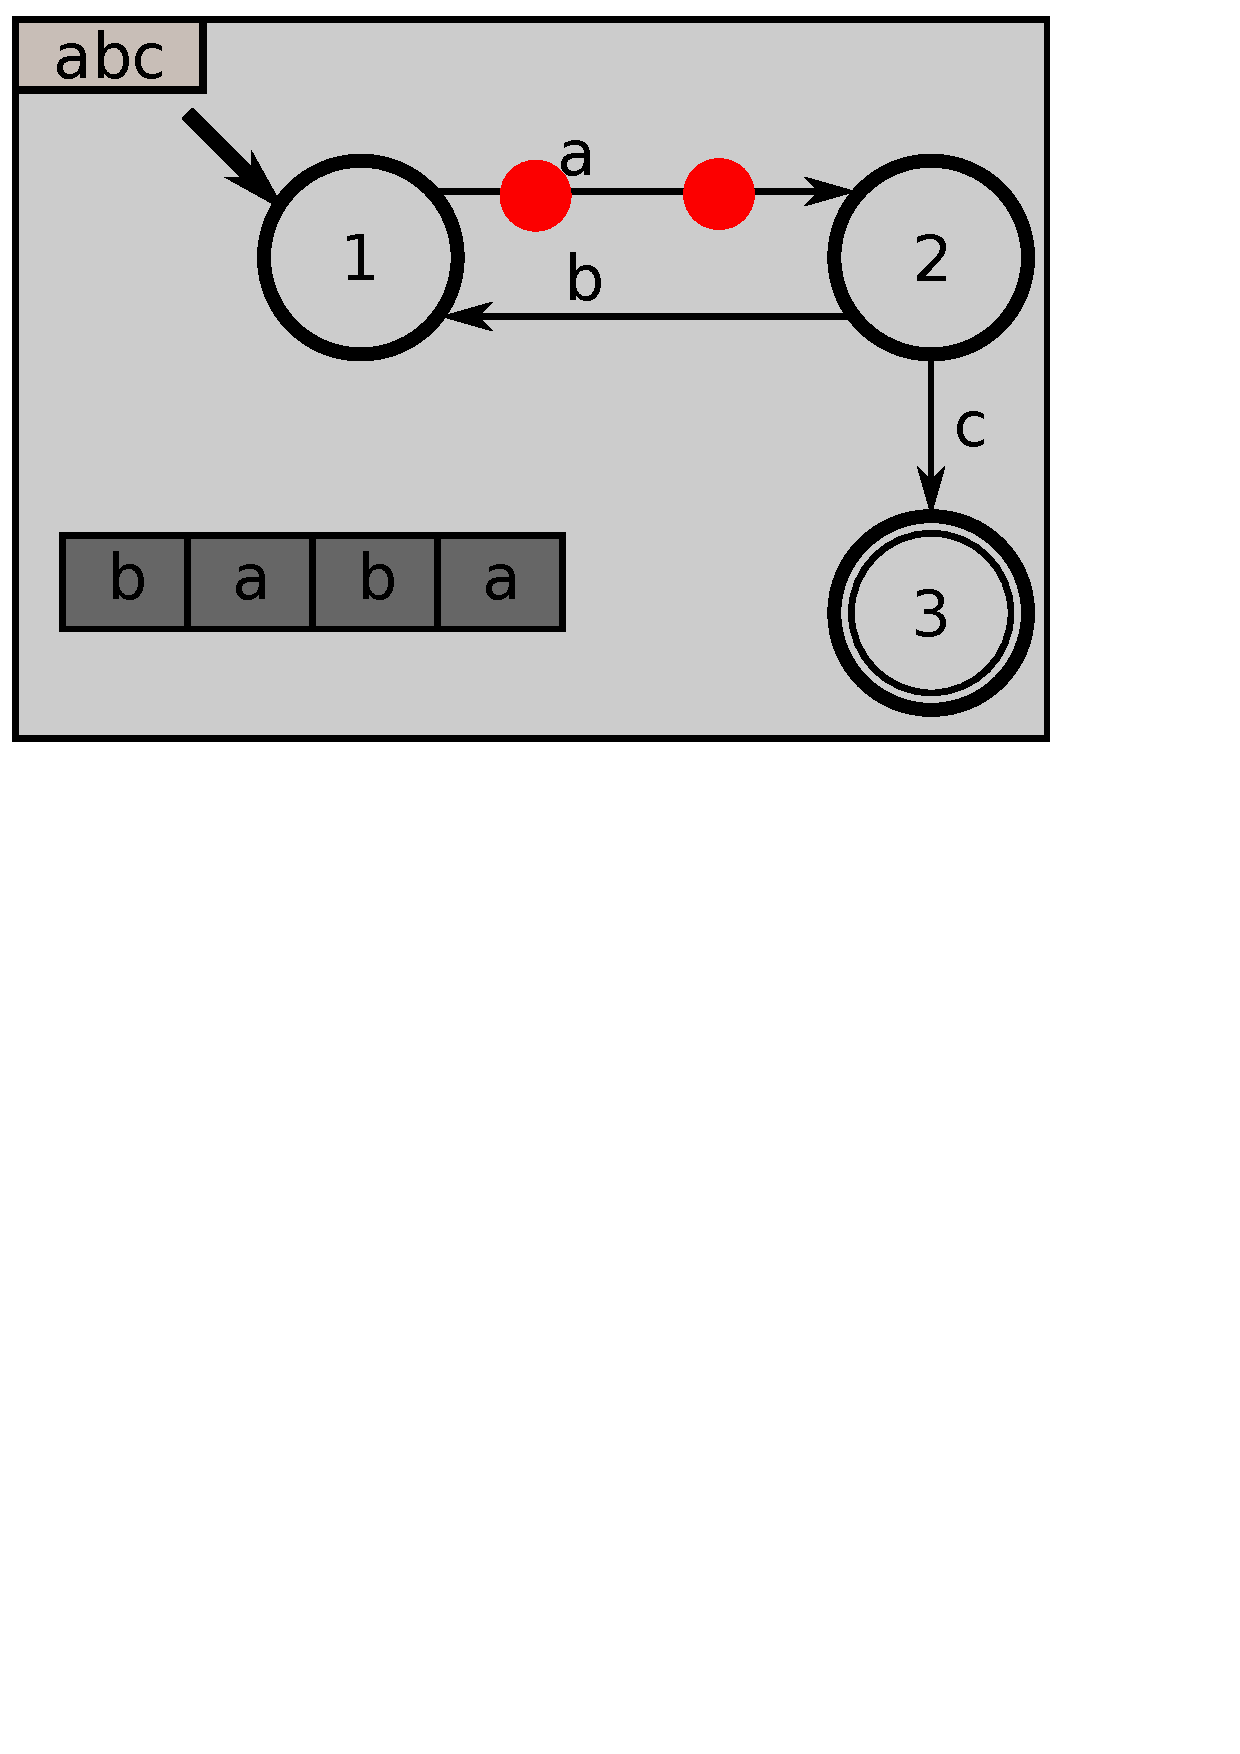
\includegraphics[width=\columnwidth, clip, trim=0cm 17cm 3cm 0cm]{FSM_MA21.pdf}%
      \caption{\textbf{Animation FSM.2:} The first phase of the animation slides
      token along the \textsf{Transition} \textsf{a} (represented here in two 
      different positions to reproduce the animation's visual effect).}
      \label{fig:FSM:Model:Animation:FSA2.1}
    \end{subfigure}
    \hfill
    \begin{subfigure}[t]{0.45\columnwidth}
      \centering
      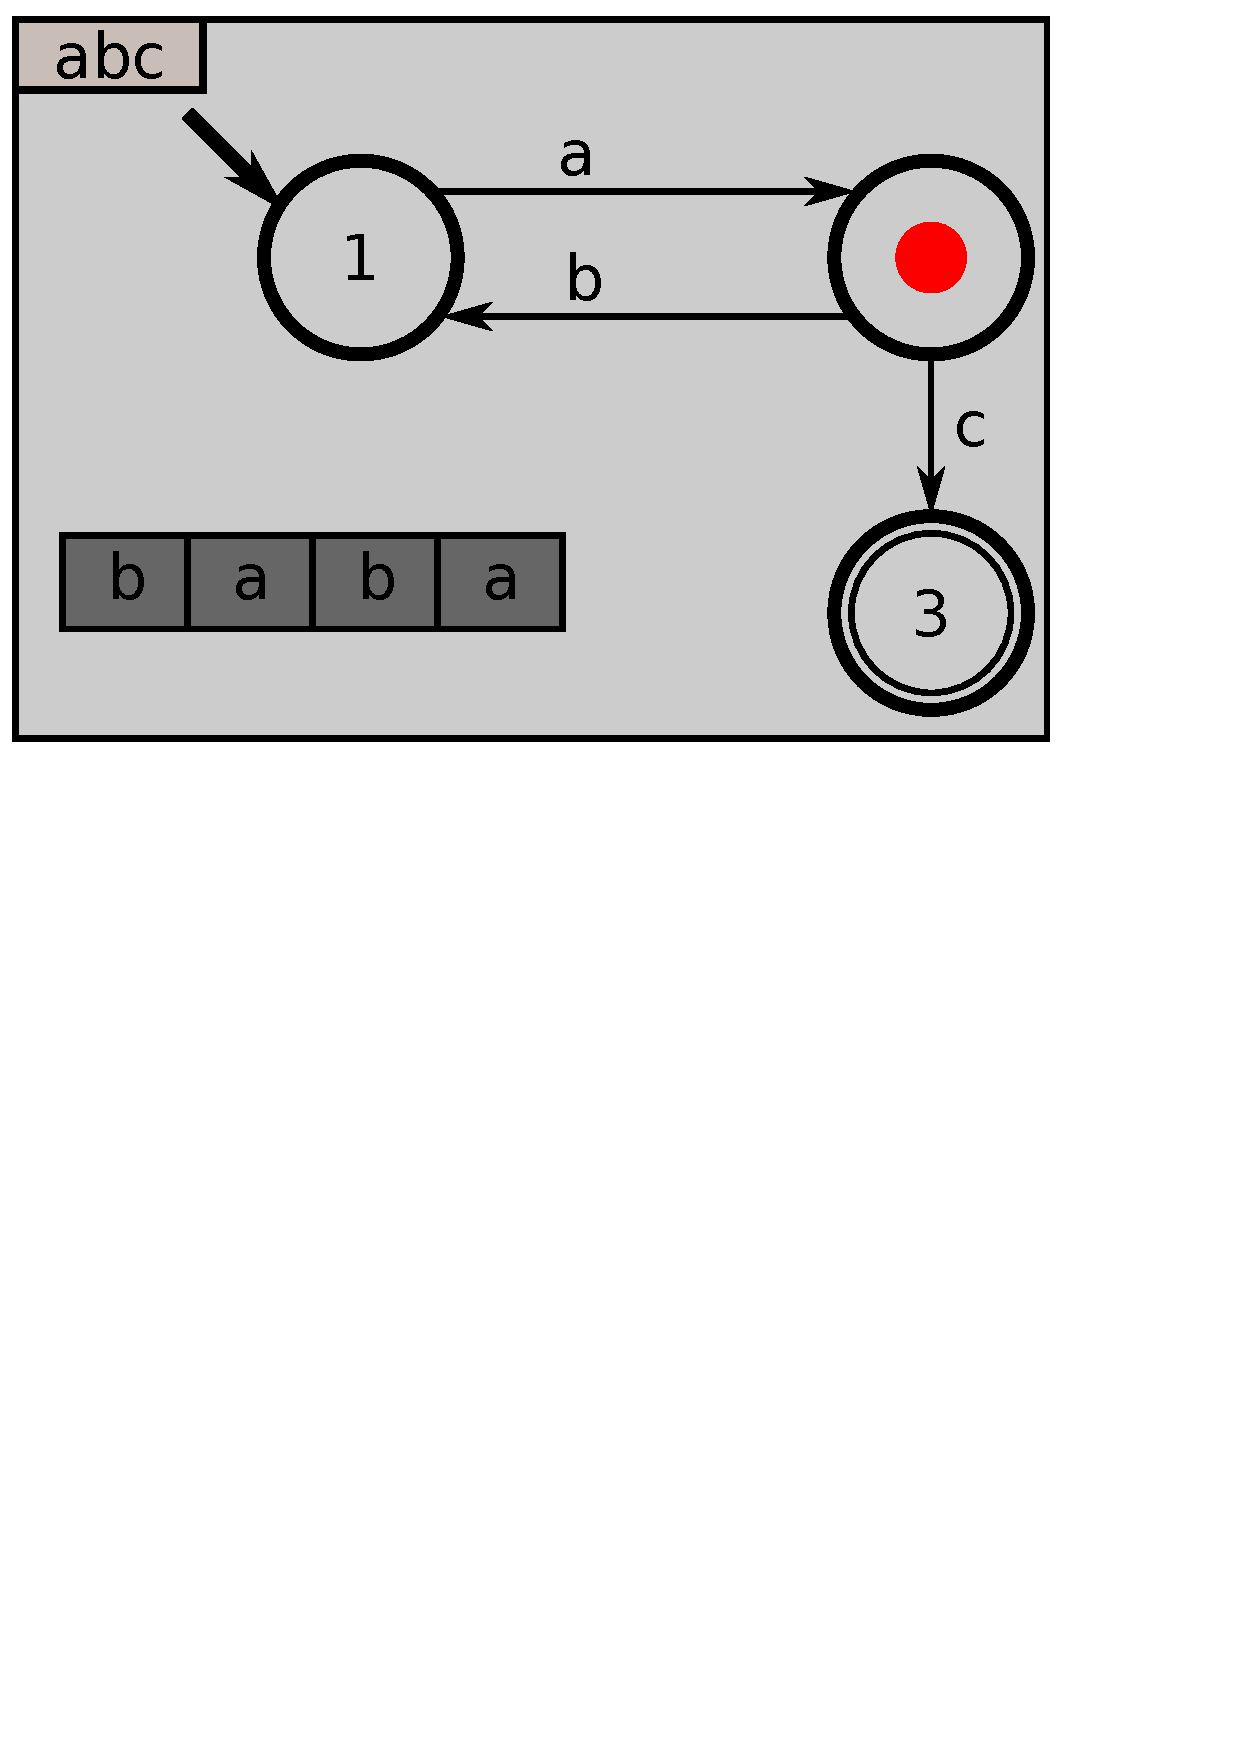
\includegraphics[width=\columnwidth, clip, trim=0cm 17cm 3cm 0cm]{FSM_MA22.pdf}%
      \caption{\textbf{Animation FSM.2:} The second phase of the animation makes
      the token appears in \textsf{State} 2, after consuming \textsf{b}.}
      \label{fig:FSM:Model:Animation:FSA2.2}
    \end{subfigure}

    \vskip\baselineskip
    \begin{subfigure}[t]{0.45\columnwidth}
      \centering
      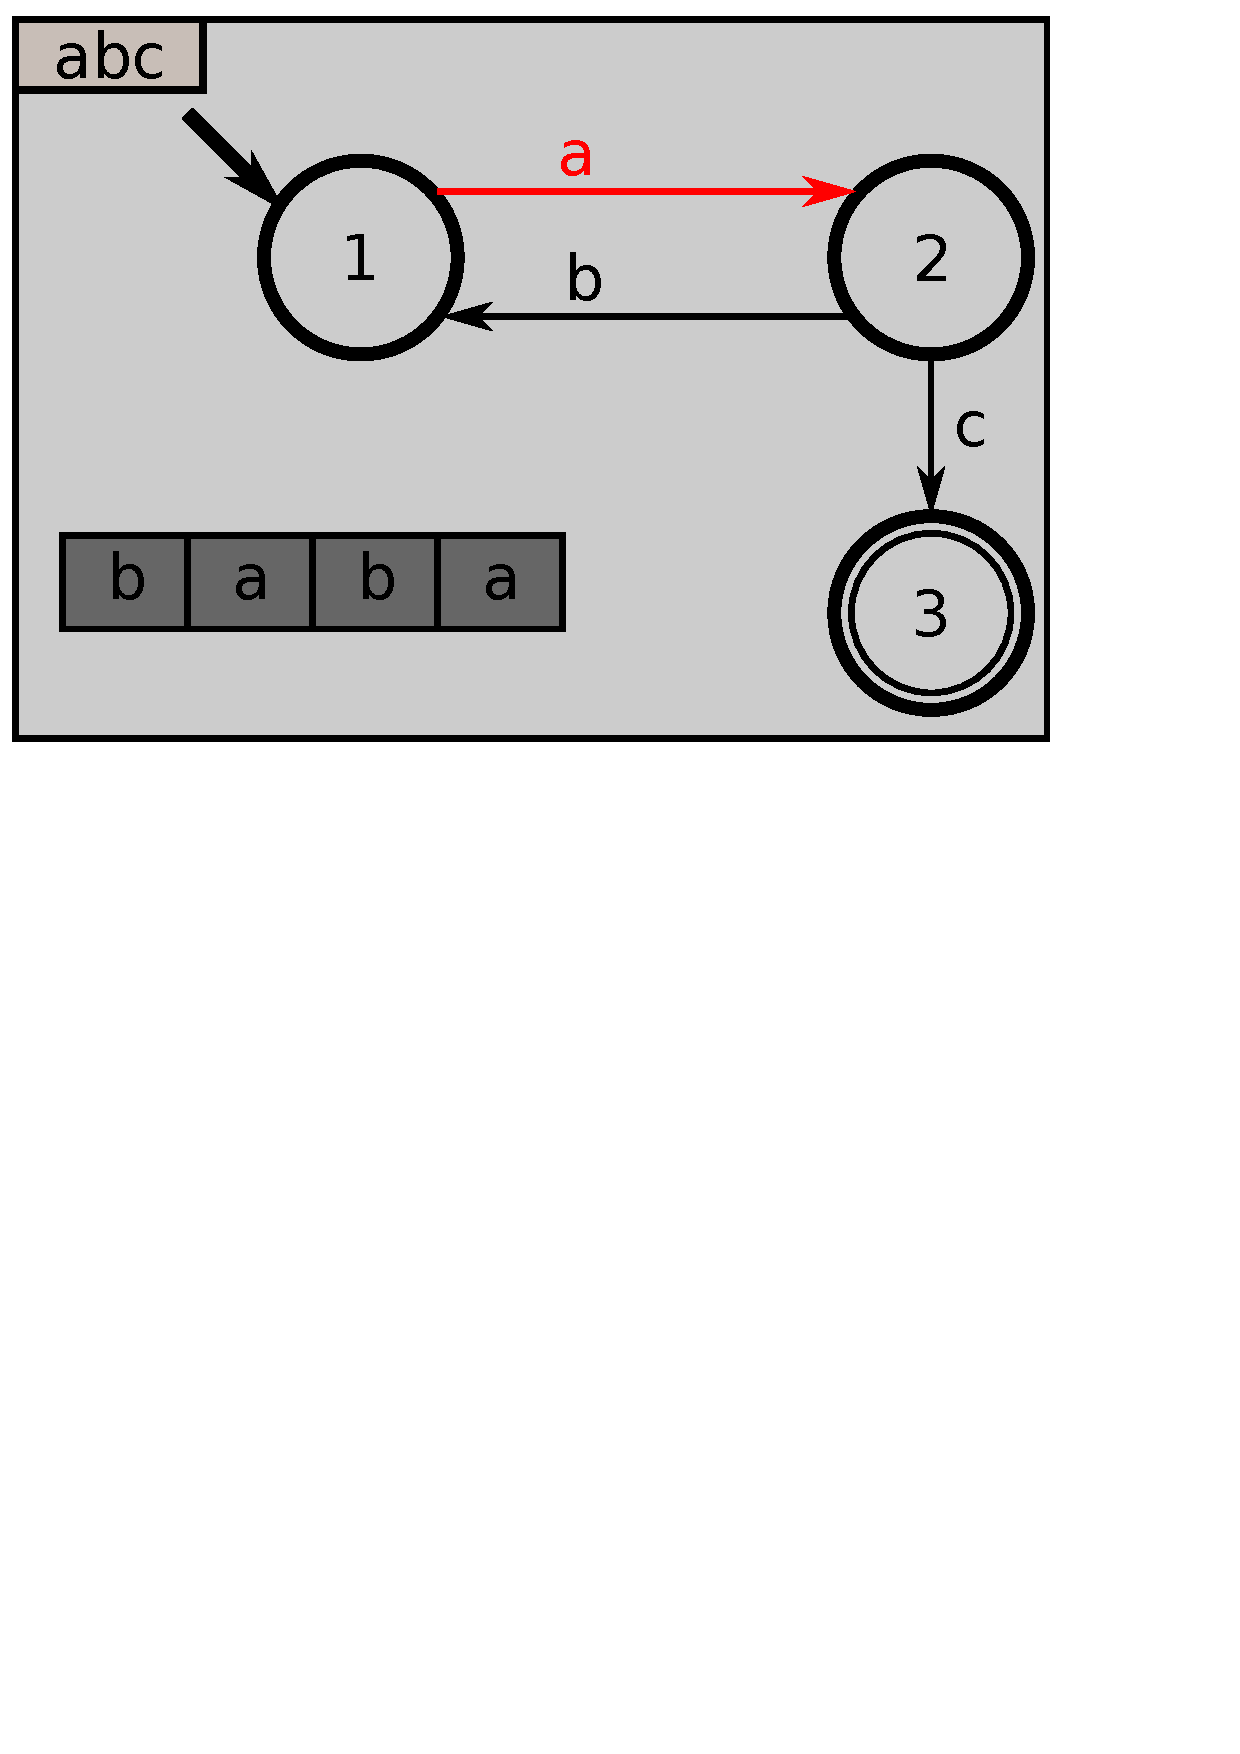
\includegraphics[width=\columnwidth, clip, trim=0cm 17cm 3cm 0cm]{FSM_MA31.pdf}%
      \caption{\textbf{Animation FSM.3:} The first phase of the animation highlights
      \textsf{Transition} \textsf{a} in red (as well as its \textsf{Trigger}).}
      \label{fig:FSM:Model:Animation:FSA2.3}
    \end{subfigure}
    \hfill
    \begin{subfigure}[t]{0.45\columnwidth}
      \centering
      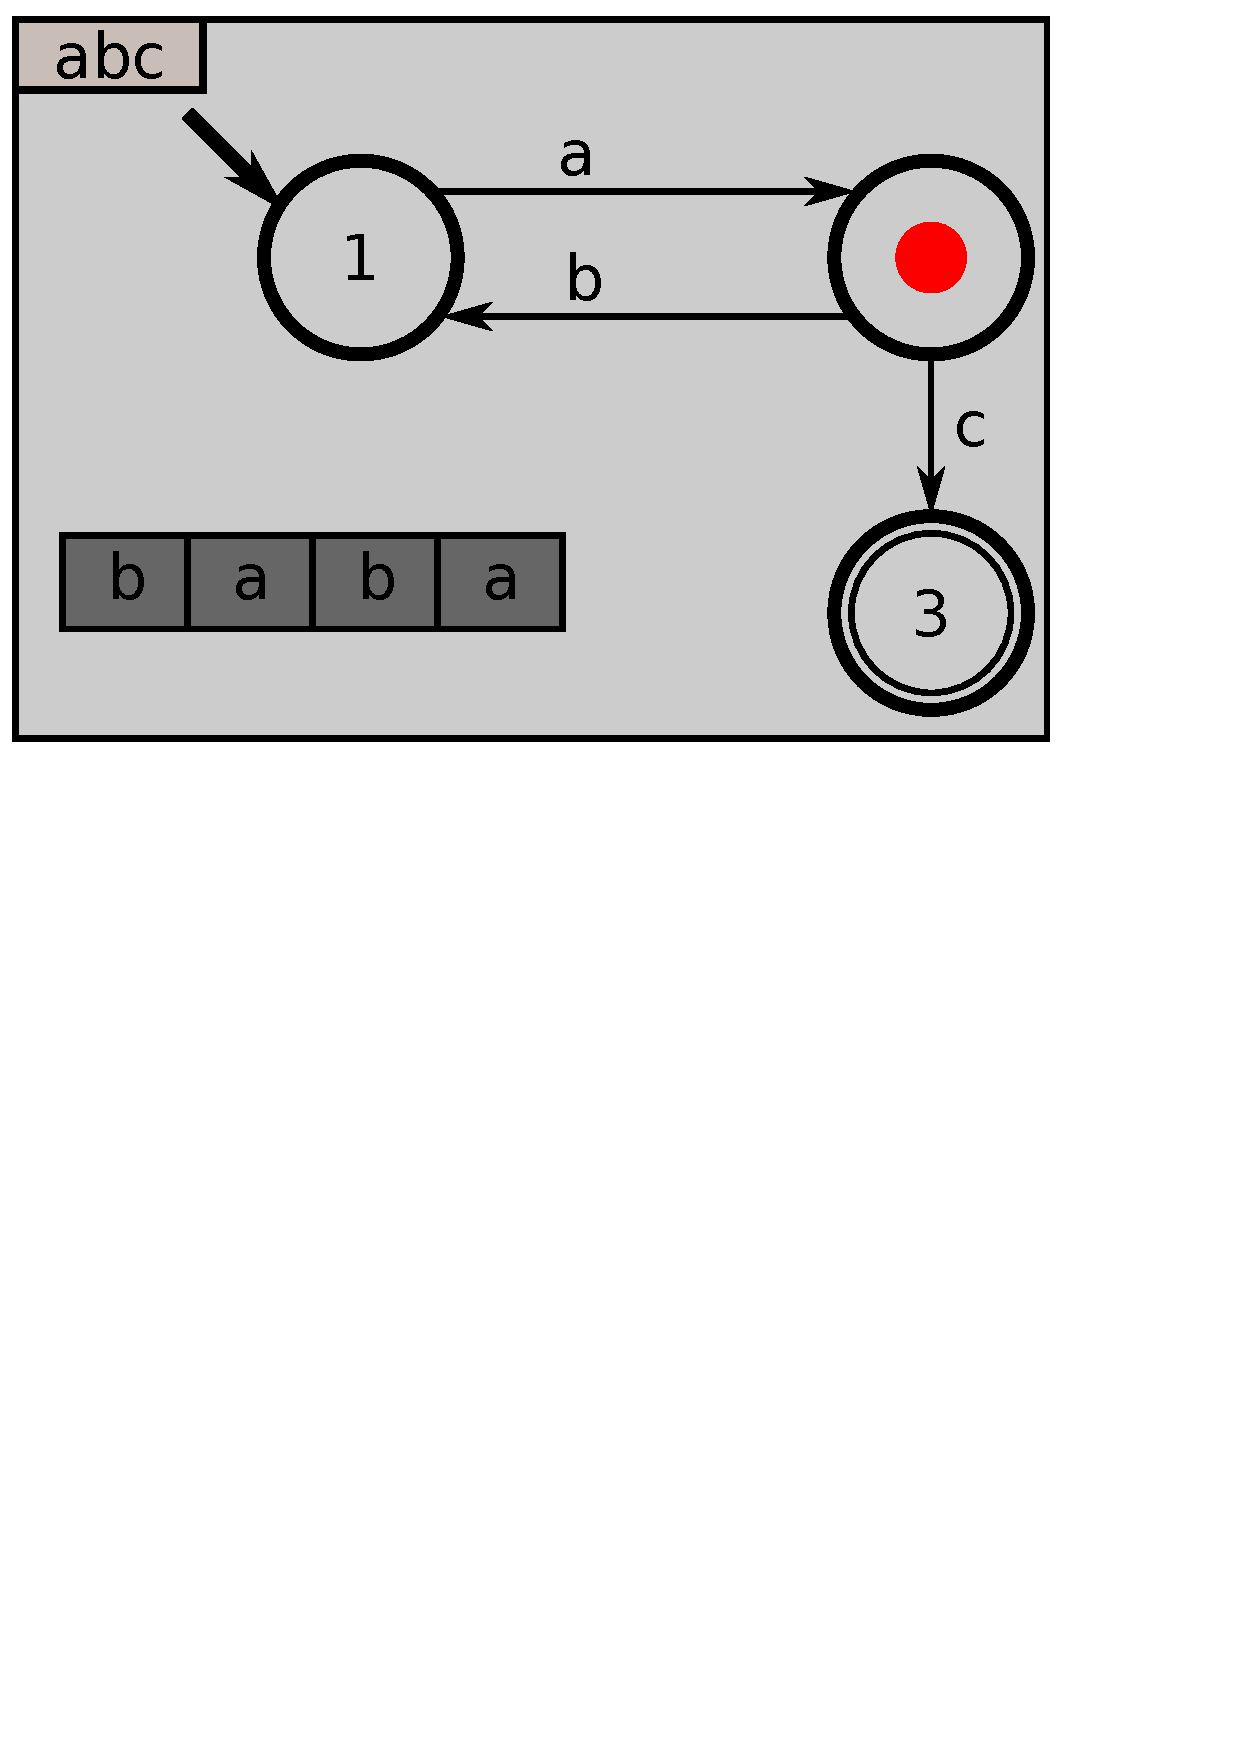
\includegraphics[width=\columnwidth, clip, trim=0cm 17cm 3cm 0cm]{FSM_MA22.pdf}%
      \caption{\textbf{Animation FSM.3:} The second phase of the animation makes
      the token appears in \textsf{State} 2, after consuming \textsf{b}.}
      \label{fig:FSM:Model:Animation:FSA2.4}
    \end{subfigure}

  \caption{\textsf{abc}: a simple model of an FSM conforming to the specification
   in \autoref{fig:FSM_MM}, and some associated animations for its execution 
   (cf. \S \ref{sec:Examples:FSM:Animations} for their specification.)}%
   \label{fig:FSM_M}%
\end{figure}


\subsection{\textsf{PN}: A \DSL for (Simple) Petri Nets}
\label{sec:Examples:PN}

\subsubsection{Specification}
\label{sec:Examples:PN:Specification}

\subsubsection{Execution}
\label{sec:Examples:PN:Execution}

\subsubsection{Animations}
\label{sec:Examples:PN:Animations}





